% Section V - Results. AI DRAFT (Claude, 2026-09-25): Kunal and advisor to edit. Every number is a macro from
% macros_counts.tex (generated by run_pipeline.py), so nothing here is typed by hand.
% Per blueprint Sec 7.5: report in aggregate; never name a study as an example of leakage.
% RESULTS OF 2026-09-25 ARE PROVISIONAL: S11 tiebreak (placeholder = rater A's code), Q20 (binary-only primary),
% Q22 (corpus closed at 18) and S05 (option B) all await the advisor. The interpretive sentences below were written
% for these numbers; if any ruling changes them, re-read every sentence marked "% RECHECK".

\subsection{Corpus characteristics}
The audit included \NincludedTotal{} studies: \NincludedWos{} from the Web of Science set and \NincludedSupp{} from the supplementary search (Fig.~\ref{fig:prisma}). Table~\ref{tab:corpus} lists each. They were published in \YearMin--\YearMax. The Mumtaz resting-state dataset was used by \DataMumtaz{} studies, MODMA by \DataMODMA, PRED+CT by \DataPREDCT{} and a private cohort by \DataPrivate; \DataOther{} used another dataset. The median sample was \NsubjMedian{} subjects (range \NsubjMin--\NsubjMax). Convolutional or recurrent networks were used in \ArchCNN{} studies and graph neural networks in \ArchGNN; Table~\ref{tab:corpus} gives each study's connectivity measure.
% REVIEW 2026-09-27 (C10): measure counts cut for space; they are in Table I.
Because several studies analyzed the same public dataset and \NgroupStudies{} came from one research group, the studies are not fully independent (Section~\ref{sec:discussion}).
% REVIEW 2026-11-07 (R2 W8, Q6): clustering by dataset and research group. POST HOC.
They fall into only \ClDatasetN{} dataset clusters, \TopDataset{} supplying \TopDatasetN{} studies and \TopDatasetEpoch{} of the \NepochTotal{} epoch-level ones, so resampling datasets rather than studies widens the interval on the epoch-level proportion below to \ClEpochDsLo--\ClEpochDsHi\% (post hoc). These proportions describe the corpus, not the literature.

\subsection{Reporting completeness by leakage surface (RQ1)}
In \PctUnclearAny\% of studies the methods did not report enough to determine whether every preprocessing step (L2--L5) was confined to the training fold (95\% CI \PctUnclearAnyLo--\PctUnclearAnyHi\%), and \PctEpoch\% partitioned at the epoch level (\PctEpochLo--\PctEpochHi\%). Fig.~\ref{fig:rq1} gives the distribution for each surface.

% REVIEW 2026-09-27 (C10): the per-surface sentences now repeat Fig. 3, which prints every count and percentage; condensed.
Connectivity was estimated from each segment or subject on its own in every study (L2). Thresholds (L3) and normalization (L4) were either not used or fit per matrix or on training data, except that normalization was not described in \PctUnclearNorm\%. Channel or band selection (L5) drew on all the data in \PctWholeSelect\% and was unclear in \PctUnclearSelect\%.
% RECHECK
The steps specific to connectivity (L2--L4) were never reported as fit on the whole dataset; leakage risk arose instead at partitioning and at selection, and the partitioning unit and the normalization step were the ones most often left undescribed.
% RECHECK
% REVIEW 2026-09-27 (C4): RQ4 moved here from Section VII so no result appears first in the Discussion.
% FIX 2026-09-27 (F4): \RqFourRho holds "$-$0.52"; inside $...$ it printed a text hyphen ("=-0.52"). Now outside math.
% REVIEW 2026-11-07 (R2 W9): exact test added and the interpretation demoted to a hypothesis. POST HOC.
In the secondary analysis (RQ4), reporting completeness fell with publication year (Spearman $\rho =$ \RqFourRho{}, 95\% CI \RqFourLo{} to \RqFourHi), but an exact test on the dichotomized measure does not support it (odds ratio \RqFourOR, Fisher's $p = \RqFourFisherP$, post hoc). From \NincludedTotal{} studies, confounded by venue and design, this is a hypothesis for a larger corpus, not a finding.

\begin{figure}[t]
\centering
\IfFileExists{figures/fig3_rq1.pdf}{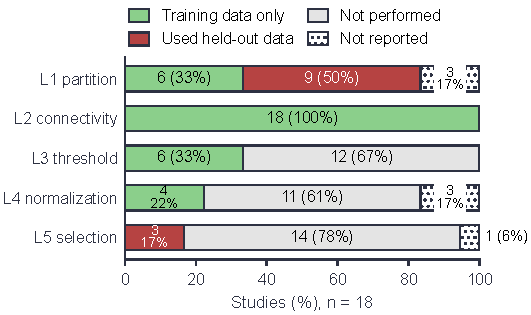
\includegraphics[width=0.95\columnwidth]{figures/fig3_rq1.pdf}}{\fbox{\parbox{0.9\columnwidth}{\centering\PENDING{Fig.~3 is generated by build\_results.py once coding is complete}}}}
\caption{Reporting completeness by leakage surface ($n = \NincludedTotal$). Segments give the number and percentage of studies in which the step was stated to use training data only, stated to use held-out data, not performed, or not reported; for L1, partitioning by subject and by epoch.}
\label{fig:rq1}
\end{figure}

\subsection{Rating distribution and agreement (RQ2)}
Before any discussion, the two raters assigned the same rating to \PctAgree\% of studies, unweighted Cohen's $\kappa = \Kappa$ (95\% CI \KappaLo{} to \KappaHi), above the pre-specified threshold of 0.4. On the individual fields they agreed on \AgreeSplit{} of \Nstudies{} studies for the partitioning unit, \AgreeScope{} for connectivity scope, \AgreeThresh{} for thresholds, \AgreeNorm{} for normalization and \AgreeSelect{} for channel or band selection.
% REVIEW 2026-11-07 (R2 W4, Q3): per-surface kappa added, post hoc. The overall kappa is dominated by the
% common L1 decisions and says nothing about the surfaces that carry the claims.
Because the overall $\kappa$ is dominated by the most common decisions, we also computed it per surface, post hoc: $\kappa = \KapLone$ (95\% CI \KapLoneLo{} to \KapLoneHi) for the partitioning unit, \KapLthree{} for thresholds, \KapLfour{} for normalization, and \KapLfive{} (\KapLfiveLo{} to \KapLfiveHi) for channel or band selection; for connectivity scope every code was identical, so $\kappa$ is undefined. The surface carrying our main result is thus the most reliably coded and selection the least: its $\kappa$ falls below the 0.4 value pre-specified for the overall rating, so every L5 figure here should be read as provisional. Disagreement concentrated there because papers compare bands or channels without saying whether the comparison chose the final model; since the rating follows fixed rules, most field-level disagreements left it unchanged.

% REVIEW 2026-09-27 (C10): duplicate of Methods condensed.
% FIX 2026-09-27 (F1): the tiebreak sentence and the post-resolution rating distribution (RQ2) were hidden behind
% the inline comment above; restored unchanged.
Studies reporting several protocols were handled as described in Section~\ref{sec:methods}. The tiebreaker resolved the remaining disagreement. After resolution, \NFree{} studies (\PctFree\%) were rated leakage-free, \NPossible{} (\PctPossible\%) leakage-possible, \NLikely{} (\PctLikely\%) leakage-likely and \NUnclear{} (\PctUnclear\%) unclear; the 95\% intervals were \PctFreeLo--\PctFreeHi\%, \PctPossibleLo--\PctPossibleHi\%, \PctLikelyLo--\PctLikelyHi\% and \PctUnclearLo--\PctUnclearHi\% respectively.

% REVIEW 2026-11-07 (R1 points 1 and 3; R2 W6, Q4): the bound on the not-reported convention. POST HOC.
\emph{How much the not-reported convention matters (post hoc).} Re-reading every unmentioned threshold, normalization or selection step as unclear rather than not performed---\StrictNcells{} coded cells---moves \StrictNchanged{} studies from leakage-free to leakage-possible, leaving \StrictNfree. The leakage-likely count is unchanged at \StrictNlikely, as is the epoch-level proportion, because both rest on what papers state rather than on what they omit. The convention cannot have inflated the central result, then, but it accounts entirely for the leakage-free count: read strictly, no study here can be verified leakage-free from its methods section.

\subsection{Accuracy by rating (RQ3)}
% RECHECK the whole subsection if the S11 tiebreak, Q20 or S05 changes the numbers. Never change a test or add a subgroup.
The primary comparison used the \NaccStudies{} studies whose recorded accuracy came from a binary depression-versus-control task; one three-class study was excluded from it and enters only the sensitivity analysis.
% REVIEW 2026-11-07 (R2 W14): the 3-versus-2 leakage-free counts reconciled explicitly in the text.
That excluded study is one of the \NFree{} rated leakage-free, which is why \NaccFree{} and not \NFree{} leakage-free studies appear in this comparison. Median reported accuracy was \MedLikely\% (IQR \IQRLikely) among the \NaccLikely{} studies rated leakage-likely and \MedFree\% (the two values were \AccFreeValues) among the \NaccFree{} rated leakage-free, a difference of \MedDiff{} percentage points (bootstrap 95\% CI \MedDiffLo{} to \MedDiffHi; Mann--Whitney $U = \MWU$, \MWp; Cliff's $\delta = \CliffDelta$, 95\% CI \CliffLo{} to \CliffHi). Across all \KWk{} strata, a Kruskal--Wallis test gave $H = \KWH$, \KWp.
The difference in medians exceeds the pre-specified smallest effect of interest of 3 points, but with only \NaccFree{} leakage-free studies, whose median is the midpoint of their two accuracies, it is not distinguishable from zero: the rank-based effect size is null and both intervals include no difference. This comparison is therefore uninformative. It is not evidence that leakage risk is associated with accuracy, nor evidence that it is not.
% RECHECK

Across sample-size terciles (small, medium, large), leakage-likely studies numbered \NLikelySmall/\NLikelyMedium/\NLikelyLarge{} and leakage-free studies \NFreeSmall/\NFreeMedium/\NFreeLarge, too few per cell to compare accuracy within terciles.
% REVIEW 2026-09-27 (C10): condensed % RECHECK
% REVIEW 2026-11-07 (R2 W2; 8-page limit): Fig. 4 (accuracy by rating) REMOVED. It plotted the comparison this
% subsection calls uninformative, and R2 W2 asked for the accuracy comparison to be demoted to a secondary
% role. Dropping it was the one content cut that both frees a float and follows the review. make_fig4_rq3.py
% and the generated PDF are untouched, so the figure can be restored in one line if the advisor prefers.

The pre-specified sensitivity analyses did not change this reading. With one study per research group ($n = \SensOneN$) and without the two weakest inclusions ($n = \SensThreeN$), Cliff's $\delta$ was \SensOneDelta{} and \SensThreeDelta; and including every task ($n = \SensTwoN$) gave $\delta = \SensTwoDelta$; in all three the interval for $\delta$ spanned $-1$ to 1. With each abstract's headline figure, only \SensFourNfree{} study was rated leakage-free, too few for any comparison.
% RECHECK

% Fig. 4 removed 2026-11-07 (see the note above). Restore by reinstating this float and the Fig. 4 reference
% in the sample-size tercile sentence.
